\newpage
\section{関連技術}
\subsection{World Wide Web}
World Wide Webはインターネット上で提供されるハイパーテキストシステムである.以降,Webと表記した場合はWorld Wide Webを指すものとする.Webはクライアントサーバモデルに基づくシステムであり,WebにアクセスするためのユーザエージェントとWebサーバがHTTP通信を行うことにより実現される.ユーザエージェントにはいくつか種類があるが,利用者による閲覧を目的としたものは特にWebブラウザと呼ばれている.Web上にあるドキュメントの記述には主にHTML~\footnote{Hypertext Markup Language}が用いられる.このWeb上のドキュメントをWebページと呼ぶ.

Webブラウザが,あるWebページへアクセスした際の基本的なフローを以下に示す.HTTPに関する詳細については後に紹介する.

\begin{enumerate}
\item WebブラウザはWebサーバにWebページを要求するためのHTTPリクエストを送信する.
\item Webサーバは受け取ったHTTPリクエストを元に要求内容を解析し,要求されたデータをHTTPレスポンスとしてWebブラウザに返す.
\item WebブラウザはHTTPレスポンスに含まれるHTMLを解析する.HTMLデータの解析は上から順に解析され,外部リソースを読み込む記述があると,基本的には逐次HTTPリクエストを送信し~\footnote{例えば,scriptタグにdefer属性を付与すると,DOMツリーの構築が終了してからリソースを取得する.詳しくは\url{https://html.spec.whatwg.org/multipage/scripting.html\#attr-script-async}を参照されたい.}取得する.
\item WebブラウザはHTMLやCSS,JavaScript,画像などのリソースの解析が完了すると,Webページを描画する.
\end{enumerate}
\subsection{HTTP}
HTTPにおいて2018年現在有効なものはHTTP/1.1とHTTP/2である.
本研究では特にこの違いについて言及しないが,HTTP/1.1を基本として論述することとする.

HTTP/1.1はRFC7230~\cite{rfc7230},RFC7231~\cite{rfc7231},RFC7232~\cite{rfc7232},RFC7233~\cite{rfc7233},RFC7234~\cite{rfc7234},RFC7235~\cite{rfc7235}で定義されているアプリケーション層のプロトコルである.HTMLやXMLによって記述されたハイパーテキストの転送を目的に仕様策定されたが,画像や音声などのバイナリ形式のデータの転送も可能である.HTTPはリクエストレスポンス型のプロトコルであるため,HTTPによる通信はクライアントであるWebブラウザが送信するHTTPリクエストと,その応答としてWebサーバが返すHTTPレスポンスの組からなる.

なお,HTTP/2に関してはRFC7540~\cite{rfc7540}にて定義されている.
\subsubsection{HTTPリクエスト}
HTTPリクエストは以下の順序で構成される.各要素は改行コード(\texttt{CRLF})で区切られている.
\begin{enumerate}
\item リクエストライン
\item ヘッダフィールド
\item CRLF
\item メッセージボディ(任意)
\end{enumerate}
HTTPリクエストの例をListing~\ref{cd-http_req}に示す.1行目はリクエストラインであり,2行目以降はリクエストヘッダフィールド,最終行が\texttt{CRLF}である.この例ではメッセージボディは存在しない.
\lstinputlisting[caption=HTTPリクエスト,label=cd-http_req]{code/http_req.txt}
\subsubsection{HTTPレスポンス}
HTTPレスポンスは以下の順序で構成される.各要素は改行コード(\texttt{CRLF})で区切られている.
\begin{enumerate}
\item ステータスライン
\item ヘッダフィールド
\item CRLF
\item メッセージボディ(任意)
\end{enumerate}
HTTPレスポンスの例をListing~\ref{cd-http_res}に示す.1行目はリクエストラインであり,2行目以降はリクエストヘッダフィールド,最終行が\texttt{CRLF}である.メッセージボディにはHTMLコンテンツが含まれていたが,紙面の都合上省略した.
\lstinputlisting[caption=HTTPレスポンス(メッセージボディ以外を抜粋),label=cd-http_res]{code/http_res.txt}
ステータスラインはHTTPバージョン,ステータスコードおよびテキストフレーズから構成される.ヘッダフィールドは複数のヘッダ名とヘッダ値の組から構成される.Webサーバはステータスコードによりリクエストの結果を通知する.ステータスコードは3桁の数字からなり,100番台は情報,200番台は成功,300番台はリダイレクト,400番台はクライアントエラー,500番台はサーバエラーを表す.
\subsubsection{HTTP Cookie}
HTTPクッキーはWebでステートフルな通信を確立することを可能とした技術である.
HTTPはステートレスなプロトコルであり,Webサーバは複数のリクエストをまたいだ情報や状態の保持を行うことができない.しかし,Webの発展に伴い,ショッピングサイトや契約した利用者のみにサービスを提供するようなセッション管理を行うニーズが発生した.そこで,セッション管理を実現するための仕組みとして,HTTPクッキーが[14] .HTTPクッキーは現在,RFC6265[15] として標準化されている. 

HTTP Cookieを利用することにより,WebサーバはWebブラウザにデータを保存させ,そのデータを次回以降のHTTPリクエストに含めさせることができる.HTTP Cookieはこのような仕組みで保存したデータをさす場合もある.
HTTP CookieはWebサーバにより発行され,Set-CookieヘッダによりWebブラウザ内にドメイン毎に保存される.
\begin{verbatim}
Set-Cookie: foo=bar
Set-Cookie: name=john; Expires=Wed, 01 Jun 2020 10:00:00 GMT
\end{verbatim}
Set-Cookieヘッダには保存するデータに加え,有効な日時(Expires属性),送信されるドメイン(Domain属性),送信されるURLの階層(Path属性),送信をHTTPSに限定するかどうか(Secure属性),JavaScriptなどからの読み込みの可否(HttpOnly属性)を指定することができる.HTTPクッキーの最大サイズは4KBであり,1ドメイン毎に最低50個(Webブラウザの実装による)のcookieを保存でき,合計で3000個のcookieを保存することができる.ただし,保存できる容量や数はWebブラウザの実装によって一部増加している.Webブラウザは保存したHTTPクッキーをCookieヘッダにより送信する.
\begin{verbatim}
Cookie: foo=bar; name=john
\end{verbatim}
\subsection{クライアント}
本節では,Webを構成する要素としてクライアントサイドの技術について解説する.
\subsubsection{Webブラウザ}
ユーザエージェントとなるソフトウエアの1つにブラウザがある.ブラウザはWebを閲覧する機能を利用者に提供する.
ブラウザは利用者の操作によりHTTP通信を行い,リソースを取得し,描画を行う.
ブラウザの主な構成要素を表~\ref{tb-browser}に示す.
\begin{table}[H]
\centering
\caption{ブラウザの構成要素}
\label{tb-browser}
\begin{tabular}{l|p{30em}}
構成要素 & 概要  \\ \hline\hline
ユーザインターフェース    & Webを閲覧する上で必要なインターフェースを提供する.戻る/進むボタン,URLの入力を受け付けるアドレスバー,ブックマークメニューなどがある.要求したWebページを表示するメインウィンドウを除くすべての部分である. \\\hline
ブラウザエンジン       & ユーザインターフェース及びレンダリングエンジン間の処理を整理する.\\\hline
レンダリングエンジン     & 要求されたコンテンツを解釈し,描画処理を行う.デフォルトでは,HTMLドキュメント,XML ドキュメント,画像を表示できる.プラグイン(またはブラウザの拡張機能)を通じて他の種類のファイルも表示できる.       \\\hline
ネットワーキング       & HTTPリクエストなどのネットワークの呼び出しに使用される.HTTP通信において,サーバからの認証要求のブラウザエンジンへの通知や,HTTPクッキーや認証情報の付加なども行う.\\\hline
JavaScriptエンジン & 取得したJavaScriptコードを解釈し,実行を行う.クロスドメイン制約に基づいて通信処理の制限も行う.\\\hline
データストレージ       & キャッシュやHTTPクッキーなど様々なデータを保存する領域.                     
\end{tabular}
\end{table}
キャッシュやHTTPクッキーなどのデータストレージに保存されたデータは,ブラウザの機能により削除することができる. 
また,多くのブラウザにはプラグインと呼ばれる,ブラウザの機能を拡張するためのプログラムをダウンロードし組み込むことができる.

StatCounter~\footnote{\url{http://gs.statcounter.com}}によると~\footnote{2018年1月の結果である.},デスクトップに限定した場合人気のあるブラウザは,Chrome,Firefox,IE,Safari,Edgeである.
以降,これらのデスクトップに限定した場合の人気のあるブラウザをメジャーブラウザと呼ぶこととする.
メジャーブラウザに関する違いを表~\ref{tb-browser_family}にまとめた.
\begin{table}[H]
\centering
\caption{メジャーブラウザの比較}
\label{tb-browser_family}
\begin{tabular}{llll}
ブラウザ    & シェア     & レンダリングエンジン & JavaScriptエンジン \\ \hline\hline
Chrome  & 65.98\% & Blink      & V8             \\\hline
Firefox & 11.87\% & Gecko      & SpiderMonkey   \\\hline
IE      & 7.28\%  & Trident    & Chakra         \\\hline
Safari  & 5.87\%  & WebKit     & JavaScriptCore \\\hline
Edge    & 4.11\%  & EdgeHTML   & Chakra        
\end{tabular}
\end{table}
これらのブラウザはほぼ同様の機能を備えているが,レンダリングエンジンやJavaScriptエンジンが異なる.
\subsubsection{HTML}
HTML~\footnote{HyperText Markup Language}はHyperTextを記述する言語仕様である.HyperTextとは,ハイパーリンクの機能を持ったドキュメントである.ハイパーリンクはあるドキュメントが別のドキュメントを単方向リンクするものである.これを発展してWebが誕生したといった背景もある.

HTMLにはいくつかのバージョンがあるが,2018年現在最新の仕様はHTML5.2~\cite{html5_2}である.HTML5のメジャーアップデートではウェブアプリケーション開発のための機能追加や文書構造の改善を図ることを目的として2014年に勧告された.マイナーバージョンアップに関しては適宜行われている.
\subsubsection{JavaScript}
JavaScriptはEcma International[18] によって仕様策定されたオブジェクト指向のスクリプト言語である.Netscape Communications社によって開発され,1997年にECMAScript[19] として標準化された.JavaScriptは主にクライアントサイドスクリプトとしてブラウザによって実行されるが,サーバサイドスクリプトとして利用される場合もある.ここではクライアントサイドのJavaScriptついて説明を行う.
JavaScriptはHTMLファイルに直接記述するか,外部ファイルとしてHTMLファイルに読み込む方法がある.JavaScriptを用いることで,ブラウザに実装されているAPIの利用やブラウザによって解釈されたHTMLのDOM(Document Object Model)操作などが行える.JavaScriptはブラウザに搭載されているJavaScriptエンジンによって解釈され実行される.JavaScriptエンジンの違いによって,処理速度の差や挙動の違いが生じるものがある.


JavaScriptはEcma Internationalによって仕様策定されたオブジェクト指向のスクリプト言語である.Netscape Communicationsによって開発され, 1997年にECMAScriptとして標準化された.JavaScriptは主にクライアントサイドスクリプトとしてWebブラウザによって実行されるが,サーバサイドスクリプトとして利用される場合もある.ここではクライアントサイドのJavaScriptついて説明を行う.

JavaScriptはHTMLファイルに直接記述するか,外部ファイルとしてHTMLファイルに読み込む方法がある.JavaScriptはWebブラウザに搭載されたJavaScriptエンジンによって解釈され実行される.JavaScriptエンジンは一般的にWebブラウザベンダによって異なるため,挙動の違いが生じるものがある.JavaScriptを用いることでWebブラウザに実装されているAPIの利用やWebブラウザによって解釈されたHTMLのDOM操作などが行える.JavaScriptはWebブラウザで実行されるため,利用者のWebブラウザに関する情報を取得する手段として有効である.

また,言語仕様とは異なり,ブラウザで利用できるJavaScript APIはWHATWGで仕様が策定されている.主要な機能はHTML5.1[20] で標準化され,さらに高機能なAPIは機能ごとに標準化されている.代表的な例としては,ブラウザでのP2P通信を実現するWebRTC API[21] や高機能なクライアントストレージを提供するWeb Storage API[22] ,位置情報を取得するGeolocation API[23] などがある. 
\subsection{サーバ}
本説では,Webを構成する要素としてサーバサイドの技術について解説する.
\subsubsection{Webサーバ}
\subsubsection{PHP}
\subsubsection{Node.js}
\subsection{オペレーティングシステム}
\subsection{CPU}
本節では本研究で対象となるCPUの機能とCPUファミリについて紹介する.
\subsubsection{SSE2}
SSE~\footnote{Streaming SIMD Extensions}は,Intel Pentium IIIプロセッサで1999年に導入されたIntel x86アーキテクチャへのSIMD命令セットの拡張である. SSEには70個の命令が含まれている.SSEが搭載されたCPUは,4つの32ビットレジスタを持ち,単精度浮動小数点データのみをサポートしている.レジスタを64ビットに拡張したSSE2は,2001年にIntel Pentium IVプロセッサで導入された.SSE2では倍精度浮動小数点データをサポートしている.このため,SSEとSSE2のプロセッサでは同じ計算であっても,計算結果に差異が生じる.
ただし,SSE3とSSE4.xはSSE2と互換性があるので,計算結果は同様である.
\subsubsection{HTT}
HTT~\footnote{Hyper-Threading Technology}は2002年にIntel Xeonプロセッサへ導入された.
複数の独立したタスクを一度に実行するSMT~\footnote{Simultaneous Multithreading}のIntelにおける実装である.
後に,Pentium 4,Itanium,Atom,Core iシリーズに導入された.HTTを使用すると,1つの物理的なコアが2つの論理プロセッサとしてOSに表示される.OSは1つの物理コアを利用して2つのプロセスを一度にスケジューリングできる.ただし物理コアの場合とは異なり,論理コアは浮動小数点演算ユニットと整数演算ユニットを共有するため,1つのプロセスが片方の演算ユニットを占有するともう1つのプロセスはその演算ユニットでの演算が行えない.つまり2つの論理コアで浮動小数点データのみを計算する場合は1つの物理コアのように機能する.
例えば,モンテカルロ法による円周率$\pi$の算出には浮動小数点と整数の両方のデータを複数回計算する.
HTTが有効なCPUにおいてこの計算を実施した場合,プロセスの処理を遅れることから識別が可能となる.
\subsection{マルチコア}
マルチコアプロセッサは2つ以上の物理演算ユニットを搭載している.キャッシュやバスを共有するので単一のCPUで並列処理を実行でき,各コアはほとんど競合を起こさずに同時に計算できる.HTTとは異なり,マルチコアプロセッサはコア数に応じて同時処理を行うスレッドを実行できる.
\subsubsection{Turbo Boost}
Turbo Boost~\footnote{Intel Turbo Boost Technology}はCPUの動作周波数を上げることでパフォーマンスを向上させる機能である.Intelが製造するCPUに実装されている.Turbo BoostはCPUの動作周波数を常に上げるのではなく,処理の内容や使用するCPUコア数,CPUの温度などの要因によって動的に決定する.また,負荷の高い処理を実行するときや複数のCPUコアを同時に使用するときはTurbo Boostが効果的に機能しない.

なお,Turbo Boostには実装された世代に応じてIntel Turbo Boost TechnologyとIntel Turbo Boost Technology 2.0の2つがあるが,提案手法が対象とするのはIntel Turbo Boost Technology 2.0のみである.以降,Turbo Boostと表記した場合はIntel Turbo Boost Technology 2.0を指すものとする.
\subsection{AES-NI}
AES-NI~\footnote{Advanced Encryption Standard New Instructions}はIntelおよびAMDのx86アーキテクチャにおける拡張命令セットであり,2010年のIntel Coreプロセッサファミリで導入された.この命令は暗号アルゴリズムAESによる高速で安全なデータの暗号化と復号が可能とする.AES-NIは,AESのハードウェアアクセラレーションを提供する6つの命令で構成されている.4つの命令はAESによる暗号化と復号をサポートし,他の2つの命令はAESによる鍵拡張をサポートする.Crypto++~\footnote{\url{http://www.cryptopp.com/}}を用いた性能解析では,Pentium 4上でAES/GCMを使用した際に,1バイトあたり約28.0サイクルから1バイトあたり3.5サイクルまで暗号操作によるクロック数が減少する.Web Cryptography APIはブラウザが稼働する端末にAES-Nが有効なCPUが搭載されている場合に限り,AES-NIによる暗号化と復号を行う.CPUがAES-NIをサポートする場合,AES-NIがサポートされていないCPUよりも高速に暗号化および復号の計算を行うことができる.

メジャーブラウザでは,Web Cryptography API~\footnote{\url{https://www.w3.org/TR/WebCryptoAPI/}}を用いたAESによる暗号化と復号処理においてAES-NIが機能するように実装されている.
\subsubsection{CPUファミリ}
\ref{tb-cpu}にIntelが提供するCPUについてまとめた.近年はマルチコア化に加えてSSE,HTT,AES-NIといった拡張機能の搭載が増加している.ほかにもTurbo Boost,Advanced Vector eXtensions(AVX),およびVT-x,VT-d,VT-cなどの仮想化技術も同様に増加している.
\subsection{アプリケーション}
\subsection{仮想化}
\subsection{統計解析}

\subsection{機械学習}
本節では,典型的な機械学習手法として,SVM~\footnote{Support Vector Machine}を紹介する.
SVMは1995年に,AT\&T社のV.Vapnikによって提案された2クラスの分類を行うための教師有り学習手法である.
与えられたデータから,クラスの境界面を決定することによって,分類するための教師データを生成する.
境界面は,マージン最大化によって決定され,クラスの境界付近に存在するデータから,可能な限り離れた位置に境界面を設置される.
図~\ref{fig-svm}に教師データにおける境界面の概念を図示する.
\begin{figure}[H]
	\centering
    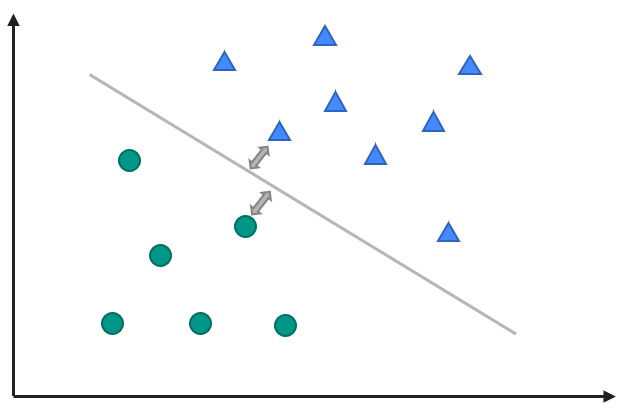
\includegraphics[width=0.6\textwidth,pagebox=artbox]{fig/svm.png}
    \caption{SVMによる分類境界面}
    \label{fig-svm}
\end{figure}
ある2次元平面上に円で表現されているデータと三角形で表現されているデータが存在する.これらのデータの境界面をSVMによって作成する場合,各クラスのデータから,他のクラスに最も近いデータを抽出し,その中間を通る面をこれら2つのクラスの境界面としている.
未知のデータを分類する際には,この境界面を利用しどちらのクラスに属するかを判断することで分類を行う.
また,入力値をそのまま扱うと境界面をとることができない場合がある.
そのような場合にも対応できるように,入力値空間から高次元空間へ写像をとりその高次元空間で境界面を作成する.

基本的には2クラス分類ではあるが,多クラス分類に対応したライブラリとしてLibSVM~\footnote{\url{https://www.csie.ntu.edu.tw/~cjlin/libsvm/}}や,SVM Light~\footnote{\url{http://svmlight.joachims.org/}}がある.
多クラスのSVMには,one-against-all方式と,pairwise方式がある.one-against-all方式では,分類データがそのクラスに属しているか否かの判定を各クラスに対して行う.学習にかかる時間は長くなるが分類性能は比較的高いとされている.
pairwise方式では複数あるクラスの内2つを選び,どちらのクラスに近いかをトーナメント方式で判定する.学習にかかる時間は比較的短いが,one-against-all方式に比べて精度は下がるとされている.